\chapter{Literature Review}\label{ch:related_work}
This chapter will center on an exploration of various pieces of literature and related works that have been thoroughly reviewed, aligning with the overarching purpose of this study.\\
To facilitate the reader, this chapter has been divided into multiple subsections, which follow the structure of this work. 

\section{Fleet and Transportation Network}
Most of the literature reviewed during the development of this study focused on (Autonomous) Mobility-on-Demand, therefore only considering human mobility.% CONSIDERA TALKING ABOUT ALSO GOODS SOMEHOW. FIND SOME PAPERS WHO DO THAT
In this case, \citepaperofs{amod_review}{Frazzoli} indentify three main mathematical models used to represent transportation networks: graph-theoretic, queuing theory and continuum models. \\
\subsubsection*{Graph-theoretic approach}
In graph-theoretic models, the transportation network is modeled as a directed graph $G  \langle V, R\rangle$, where $V$ is the set of vertices and $E\subseteq  V \times V$ is the set of edges. Usually, each node $v \in V$ represents a location, or a station. In \cite{project_thesis}, in a more abstract way, nodes are used to represent areas of interest. Each edge $\langle v_1, v_2\rangle \in E$ rapresents a connection, which could be a road or a collection of those, from $v_1$ to $v_2$. Furthermore, each link is usually associated with a metric, such as distance $d : E \rightarrow R_{\ge0}$.  Many studies adopt a dynamic fluid approach, representing AVs and customers not as individual entities but rather as flows moving between nodes. In this framework, models that do not vary with time often simplify to static network flow problems. Alternatively, graph-theoretic models can be integrated with vehicle-centric models, where both AVs and customers are modeled individually.
\subsubsection*{Queuing-theoretic approach}
Queuing theory is concerned with the examination of waiting lines. In the context of AMoD systems, trips are conceptualized as queues between locations, enabling the analysis of various characteristics AVs, closely linked to waiting times. Formally, considering N stations situated at specific geographical locations with m AVs providing mobility services. Customers arrive at each station based on an exogenous stochastic process (usually a Poisson process with rate $\lambda$, like for example in \cite{queue_theory}) and select destinations with certain probabilities. If AVs are accessible at a station, customers proceed to their respective destinations; otherwise, they exit the system (referred to as passenger loss). Travel times between stations are also stochastic and are typically modeled as exponentially distributed random variables. When formulating policies for AMoD systems, the focus lies in analyzing and regulating the movement of AVs from one queue to another.
These models are commonly employed in time-invariant settings. The scenario of infinitely large fleets  has garnered particular attention for deriving theoretical insights.


%The transportation network is modeled as a directed graph G = ⟨V , E ⟩, where V is the set of vertices and E ⊆ V × V is the set of edges (Figure 3a). A node v ∈ V represents a location, such as a station or an urban area, and an edge ⟨v1 , v2 ⟩ ∈ E represents a road (or a combination of roads) from location v1 to location v2. Each edge is usually associated with metrics such as travel time t : E → R≥0 and distance d : E → R≥0 [e.g., tij := t(i, j) is the travel time of edge ⟨i, j⟩].
\subsubsection*{Battery model}
This chapter delves into the exploration of various sources and solutions that have been examined in the development of the battery model utilized in this study. As the first work considered, \citepaperofs{MONTOYA201787}{Montoya} employed linear piece-wise approximations to approximate the nonlinear charging function, reporting an error of approximately 1\%. Additionally, they introduced the concept of different types of charging stations. \citepaperofs{froger2022electric}{Froger} and \citepaperofs{kancharla2020electric}{Kancharla} also employed piece-wise linear functions for their respective charging regimes. Conversely, \citepaperofs{9945248}{Nie} did not consider the possibilities for vehicle recharging in their model.\\
In terms of modeling the battery charging profile, diverse approaches have been proposed. \citepaperofs{electronics9081277}{Han} developed a model based on the internal resistance and voltage of the battery; however, this model was disregarded in favor of others that better captured the battery charging profile based on more relevant factors. \citepaperofs{8115230}{Yu} proposed a sophisticated model for charging constraints in general. Although their approach differs from the one presented in this work, as it incorporates charging during routing, this aspect was excluded in favor of an alternative approach. \citepaperofs{lee2020model}{Lee} considered a simplified battery model that provides states of charge (SoC) as a function of the charging current. The author asserted the general applicability of their approach to every charging profile, provided SoC(t) is a concave and non-decreasing function with SoC(0) = 0, and an inverse function $\text{SoC}^{-1}(a)$ exists for $0 < a < Q$.\\
\section{AToD Challanges}

\subsubsection*{AV Dispatching}
For the vehicle dispatching problem, multiple solutions have been already proposed. For example, \citepaperofs{VASCO2016118}{Vasco} model it as a linear minimum cost multicommodity flow problem; \citepaperofs{holzi}{Holzapfel} model it as a MIP problem. Others, on the other hand, make use of other heuristics. For example, \citepaperofs{LEVIN2017373}{Levin} and \citepaperofs{nn_mora}{Mora} use nearest neighbors. Recently, to improve real-time capabilites, some approaches have been proposed which make use of deep learning, like for e.g. the one proposed by \citepaperofs{8693516}{Yu}.\\

\subsubsection*{AV Routing}
On a basic level, the routing problem can be reconducted to the Vehicle Routing Problem (VRP) (a thorough analysis and explanation can be found in \cite{doi:10.1137/1.9780898718515}). Usually, the VRP is solved and analyzed as a static problem, which implies that requests are known in advance. As a result, origins and destination of each trip is also known a priori. As pointed out by \citepaperofs{amod_review}{Frazzoli}, in AToD systems requests are dynamic, meaning they are not known in advance. More specifically, the task of managing an AToD system can be viewed as a specific case of the dynamic one-to-one pickup and delivery problem. As pointed out by \citepaperof{zhang2016}{Zhang},to provide a more detailed characterization of these systems, several additional attributes and constraints must be considered:
\begin{itemize}
	\item Immediate Service Requests: Requests are made for immediate service rather than being scheduled in advance with specified time windows.
	\item Stochastic Customer Arrivals and Travel Times: The timing of customer requests and the duration of travel are subject to stochastic variability.
	\item Multi-Occupancy Vehicles: Contrary to \cite{zhang2016}, vehicles must be considered to have a capacity, rather than being single-occupancy. This is motivated by the fact that recently developed AV are equipped with more than one seat (see for e.g. \cite{dlr-nemo-bili})
\end{itemize}

\citepaperofs{9294258}{Wollenstein-Betech} propose a solution to the routing-rebalancing problem in mixed traffic situations. They propose an interesting two-graph solutions, i.e. one graph for the AToD system and one for the pedestrians which are interconnected. Furthermore, they also consider private and public vehicles. \\
\citepaperofs{pavone2012robotic}{Pavone} also propose a solution for the rebalancing problem. Although they mainly consider MoD systems, their approach can be easily applied to AToD systems. Their solution, moreover, focuses only on the rebalancing issue, which is studied using a steady-state fluid model, as pointed out in \cite{9294258}. Furthermore, this work does not take into consideration congestions in their model. \\

\subsubsection*{AMoD Rebalancing}
In the context of network flow models, rebalancing is usually formulated as a (integer) optimization problems, such as in the works of \citepaperofs{8917521}{Zgraggen}, \citepaperofs{8938759}{Carron} and of \citepaperofs{6580187}{Smith}. Crucially, in real-time texting, the rebalancing problem is solved leveraging the model-predictive control framework, such as in the works mentioned above. \\
\citepaperofs{9304517}{Wollenstein-Betech} investigate effective pricing and rebalancing strategies for AMoD systems from a macroscopic planning standpoint. It aims to optimize profits while ensuring system load balance. Using a dynamic fluid model, the study demonstrates equilibrium attainment via pricing policies and develops an optimization framework for determining optimal pricing and rebalancing approaches. They model customers and vehicles located in regions using a queuing approach, i.e. two queues per region representing vehicles and clients. \\
\citepaperofs{Salaza2019Cong}{Salazar} study the rebalancing problem while considering two important aspects, namely mixed traffic and congestions. The first is treated by modeling the road network and the walking network as two separate entites, which combined make up a supernetwork defining the entire transportation network. The latter are treated according to the Bureau of Public Roads (BPR) model (\cite{BPR1964}) , more specifically by approximating their model linearly. The BPR model of congestions can be expressed by \equaref{eq:bpr_model} and is visualized in \figref{fig:bpr_models_approx} as a black dotted line. 
\begin{figure}[t]
	\centering
	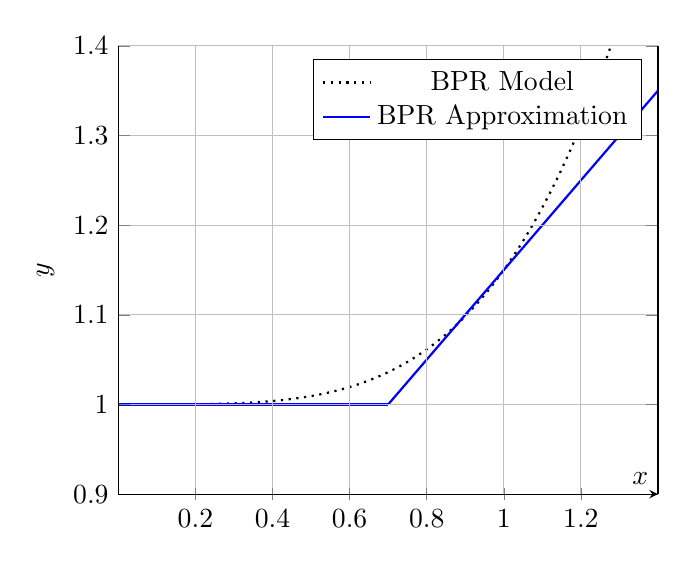
\begin{tikzpicture}
		\begin{axis}[
			xlabel={$x$},
			ylabel={$y$},
			domain=0:1.4, % adjust the domain based on your preference
			samples=100,
			grid=both,
			axis x line=middle,
			ymin=0.9, % Set the minimum y-axis value
			ymax=1.4, % Set the maximum y-axis value
			axis on top,
			legend pos=north east
			]
			\addplot[dotted, black, thick] {1 + 0.15*x^4};
			\addlegendentry{BPR Model}
			
			% Piecewise function
			\addplot[blue, thick, domain=0:0.7] {1};
			\addplot[blue, thick, domain=0.7:1.4] {1 + 0.5*(x-0.7)};
			\addlegendentry{BPR Approximation}
		\end{axis}
	\end{tikzpicture}
	\caption[BPR Model and Approximation]{BPR Model and its Approximation as a piecewise linear function. In this example, $x_{th} = 0.7$,$x_{max} = 1.4$, $a=1$, $b = 0.5$ }
	\label{fig:bpr_models_approx}
\end{figure}

\begin{equation}
	f_{BPR}(x) = 1 + 0.15x^4 
	\label{eq:bpr_model}
\end{equation}

Since this model would lead to an unconvex, i.e. intractable, problem, the authors propose a piece wise approximation of it, which take the form expressed in \equaref{eq:model_bpr_approximation}
\begin{equation}
	y = \begin{cases}
		a \quad\quad &\text{if } x\in[0,x_{th}]\\ 
		a + b\cdot(x - x_{th}) \quad\quad &\text{if }x\in[x_{th}, x_{max}]\\ 
	\end{cases}
	\label{eq:model_bpr_approximation}
\end{equation}
where $a$ and $b$ are used to model the height of the horizontal line and the slope of the second line, $x_{th}$ is the threshold of the piecewise approximation and $x_{max}$ defines the approximation window. This approximation can be seen in \figref{fig:bpr_models_approx} as a blue line. \\
\equaref{eq:model_bpr_approximation} is then used to calculate the traverse time for each edge. While this is a more representative congestion model than the one proposed in this paper in \secref{sec:vc_model}, one might argue that the two serve two different purposes. While the one proposed in \cite{Salaza2019Cong} serves to express the travel time in terms of the amount of vehicles currently traveling on the node, the one proposed in this work is used to simply limit the amount of vehicles
traveling on the link to avoid situations of stop-and-go traffic. Furthermore, it is worth mentionining that this model can be easily integrated into the model by modifying the definition of the travel time function. \\
In the abovementioned study, the energy consumption of the AVs is also modeled differently compared to this work. Within their network graph G, the energy consumption of each AV with efficiency $\eta$ traveling through arc $(i,j)$ with distance $d_{ij}$ is expressed as:
\begin{equation}
e_{ij} = (\dfrac{\rho_a}{2}\cdot A_f \cdot c_d \cdot v_{ij} + c_r \cdot m_v \cdot g)\cdot \dfrac{d_{ij}}{\eta_{\text{AV}}} \quad \forall (i,j) \in G
\end{equation}
where the aerodynamic drag is determined by the air density $\rho_a$, the frontal area $A_f$,  the drag coefficient $c_d$ and the moving velocity $v_{ij}$. The friction of the wheels on the road is determined by the rolling friction coefficient $c_r$, the mass of the vehicle $m_v$, and the gravitational acceleration $g$. \\ 
This is a more vehicle-based approach compared to the one adopted in this work, which only considers the battery dischargment, as it takes into consideration various other aspects such as drag and rolling friction. For the purpose of this work, however, it has been chosen to neglect those factors, which could be later introduced into the battery-dischargment model, to favour a more simplistic approach. Furthermore, given that in the aforementioned paper is assumed to have constant velocity $v_{ij} = \dfrac{d_{ij}}{t_{ij}}$, one can trivially adopt a similar solution for the model in this paper by making the same assumption. \\
\citepaperofs{8593743}{Wallar} tackle the rebalancing problem independently from any other AToD challenge, while also considering ride-sharing possibilities. The main idea of the propsed approach is to assign free vehicles to regions, which are computed offline, according to the estimations of traveling request per region. In this case, the requests are estimated using the particle filter. Furthermore, the division in region for the graph is formulated as an integer linear programming problem using a rechebaility matrix $R$, which indicates whether a station $j$ if recheable from $i$ within a maximum time $t_{max}$ ($R_{ij} = 1$ else $R_{ij} = 0$). Cleverly, the authors also took into consideration the fact that, although a vehicle is free, it requires some time to reach the assigned rebalancing region. In other words, if a vehicle requires eight minutes to reach a certain region, considering a time horizon of ten minutes, it will be available only for two minutes, i.e. 20\% of the time. This is used to limit the oversaturation of vehicles in the respective rebalancing regions.  

\subsection*{OThers}
\citepaperofs{8883370}{Fehn} modeled a fleet according to energy prices.